\documentclass{beamer}

\mode<presentation> {
	\usetheme{Madrid}
	\usecolortheme{rose}
	
	%\setbeamertemplate{footline}
	%若要删除所有幻灯片中的页脚,请取消注释此行
	
	%\setbeamertemplate{footline}[页码]
	%若要用简单的幻灯片计数替换所有幻灯片中的页脚,请取消注释此行
	
	%\setbeamertemplate{导航符号}{}
	%要删除所有幻灯片底部的导航符号,请取消注释此行
}

\usepackage{graphicx} % 允许包含图像
\usepackage{booktabs} % 允许在表中使用\toprule、\ midrule和\ bottomrule
\usepackage[UTF8,noindent]{ctexcap}  % 使用中文输入及显示
\usepackage[bookmarks=true]{hyperref}
\usepackage{amsmath,amssymb,bm}
\usepackage{amsthm}
\usepackage{tikz}
\usepackage{graphicx}
\usepackage{hyperref}
%\usepackage{zhlipsum}
\usepackage{algorithm,algorithmic}
\usetikzlibrary{positioning, shapes.geometric}
\newtheorem*{mathmodle}{数学模型}
%\newtheorem*{definition}{定义}

%-----------------------------------
%	以下为正文
%-----------------------------------

\title{数值函数优化方法和多目标优化} 
% 简短标题显示在每张幻灯片的底部,完整标题仅在标题页上

\author{何宇青} % Your name

\date{2024年9月25日} % 日期,可以更改为自定义日期

\begin{document}
	
	\begin{frame}
		\titlepage % 将标题页打印为第一张幻灯片
	\end{frame}
	\begin{frame}
		\frametitle{为什么需要遗传算法}
		\begin{itemize}
			\item 在函数是连续,可求导,低阶的简单情况下可解析地求最优解外,大部分情况下,只能通过数值方法求近似最优解.
			\item 至今还没有一种既能处理各种不同的复杂函数,有具有良好求解结果的数值计算方法
			
		\end{itemize}
		需要研究出一种能够在可接受的时间和可接受的精度范围内求出数值函数近似最优解的方法或通用框架,遗传算法提供了一种求解这类优化问题的通用框架.
	\end{frame}

	%------------------------------------------------
	\subsection{Subsection Example 2}
	
	\begin{frame}
		\frametitle{评价遗传算法性能的指标}
	\begin{definition}
		在环境$e$下策略$s$的在线性能$X_e(s)$定义为:
		\begin{displaymath}
			X_e(s)=\frac{1}{T}\sum_{t=1}^T f_e(t)
		\end{displaymath}
		其中$f_e(t)$是在环境$e$下在时刻$t$的平均目标函数或平均适应度.
	\end{definition}
	算法的在线性能指标表示算法从开始运行一直到当前为止的时间段内性能平均值,反映了算法的动态性能.
	\end{frame}
	\begin{frame}
		\frametitle{评价遗传算法性能的指标}
	\begin{definition}
		在环境$e$下策略$s$的离线性能$X_e^*(s)$定义为:
		\begin{displaymath}
			X_e^*(s)=\frac{1}{T}\sum_{t=1}^T f_e^*(t)
		\end{displaymath}
		其中$f_e^*(t)$是在环境$e$下在时间段$[0,t]$内最好目标函数或最大适应度.
	\end{definition}
	算法的离线性能表示算法运行过程中各代的最佳性能值的累积平均,反映算法的收敛性能.
	\end{frame}
	\begin{frame}
		\frametitle{算法性能测试函数}
		\begin{definition}[De Jong 函数F1]
			\begin{eqnarray*}
				&f_1(x_1,x_2,x_3)=\sum_{i=1}^{3} x_i^2\\
				&-5.12\le x_i \le 5.12 \,\,\,i=1,2,3
			\end{eqnarray*}
		\end{definition}
		一个简单的平方和函数,只有一个极小点$f_1(0,0,0)=0$
	
	
		\begin{definition}[De Jong 函数F2]
			\begin{eqnarray*}
				&f_2(x_1,x_2)=100(x_1^2-x_2)^2+(1-x_1)^2\\
				&-2.048\le x_i \le 2.048 \,\,\,i=1,2
			\end{eqnarray*}
		\end{definition}
		具有一个全局最小点$f_2(1,1)=0 $,该函数虽然是单峰函数,但他是病态的,难以全局极小化.
		
		
	\end{frame}
	\begin{frame}
		\frametitle{算法性能测试函数}
	\begin{definition}[De Jong 函数F3]
		\begin{eqnarray*}
			&f_3(x_1,\cdots,x_5)=\sum_{i-1}^{5}[x_1]\\
			&-5.12\le x_i \le 5.12 \,\,\,i=1,2,3,4,5		
		\end{eqnarray*}
		$[\,\cdot \,]$为向下取整函数
	\end{definition}
不连续,对于$x_i\in [-5.12,-5]$区域的每个点,都取全局极小值$-30$
		\begin{definition}[De Jong 函数F4]
			\begin{eqnarray*}
				&f_4(x_1,\cdots,x_{30})=\sum_{i=1}^{30} ix_i^4 +\textbf{Gauss}(0,1)\\
				&-1.28\le x_i \le 1.28 \,\,\,i=1,2,\cdots,30
			\end{eqnarray*}
		\end{definition}
	不考虑噪音影响时,有全局极小值$f_4(0,0,\cdots,0)=0$
	\end{frame}
	\begin{frame}
		\frametitle{算法性能测试函数}
	\begin{definition}[De Jong 函数F5]
		\begin{eqnarray*}
			&f_5(x_1,x_2)=0.02+\sum_{j=1}^{25} 1/[j+\sum_{i=1}^{2} (x_i-a_{ij})^6]\\
			&-65.536\le x_i \le 65.536 \,\,\,i=1,2 \\
			&[a_{ij}]=\\
			&\left[
				\begin{array}{ccccccccccc}
					-32 & -16 & 0 & 16 & 32 & -32 & -16 & \cdots &0 & 16 & 32\\
					-32 & -32  & -32 & -32 & -32 & -16& -16 & \cdots & 32& 32& 32
				\end{array}
			\right]
		\end{eqnarray*}
	\end{definition}
	这是一个多峰函数,共25个局部极小点,其中只有一个全局极小点$f_5(-32,-32)=0.998$
		
	
	\end{frame}
	\begin{frame}
		\frametitle{研究方法}
		\begin{itemize}
			\item \textbf{编码方法}: 二进制编码符号串表示个体
			\item \textbf{算法的影响参数}: \begin{itemize}
				\item 群体大小$M$
				\item 交叉概率$P_c$
				\item 变异概率$P_m$
				\item 代沟$G$($0<G<1$指子代与父代之间的重叠程度)
			\end{itemize}
			\item \textbf{算法种类}: \begin{itemize}
				\item 基本遗传算法(比例选择,单点交叉,基本位变异)
				\item 保留最佳个体模型
				\item 期望值模型
				\item 排挤因子模型
				\item 广义交叉模型
			\end{itemize}
		\end{itemize}
	\end{frame}
	\begin{frame}
		\frametitle{结论}
	\begin{itemize}
		\item 群体的规模越大,遗传算法的离线性能越好,越容易收敛.
		\item 规模较大的群体,遗传算法的初始在线性能较差,规模较小的群体相反.
		\item 变异概率的增大会增加群体的多样性,但降低了算法的离线性能和在线性能,并随着变异概率的增大,算法性能越接近随机搜索的性能.
		\item 使用保留最佳个体模型或期望值模型的算法比基本遗传算法的性能有明显改进.
		\item 广义交叉算子会随着交叉点的增加降低算法的在线性能和离线性能.
	\end{itemize}
	\end{frame}
	\section{多目标优化}
		\begin{frame}
			\frametitle{介绍}
			使多个目标在给定区域都尽可能地好的优化
			\begin{mathmodle}
				\begin{eqnarray*}
					&\textbf{V-min} \,f(x)=[f_1(x),f_2(x),\cdots,f_p(x)]^T\\
					&\textbf{s.t.} \left\{\begin{array}{c}
						x\in X\\
					X \subseteq \mathbb{R}^m 
					\end{array} \right.
				\end{eqnarray*}
				\textbf{V-min}表示向量最小化.
			\end{mathmodle}
		很多情况下各个子目标可能相互冲突,一个子目标的改善往往以其他子目标的恶化为代价.
		\end{frame}
	\begin{frame}
		\frametitle{最优解}
	\begin{definition}
		$X\subseteq \mathbb{R}^m $是多目标优化模型的约束集,$f(x)\in \mathbb{R}^p $是多目标优化时的目标向量目标函数,$x_1,x_2\in X$,若$f_k(x_1)\le f_k(x_2), \,\, \forall k=1,\cdots,p$,且$f_k(x_1)< f_k(x_2), \,\, \exists k=1,\cdots,p$ ,则称$x_1$优于$x_2$.
	\end{definition}
	\begin{definition}
		$X\subseteq \mathbb{R}^m $是多目标优化模型的约束集,$f(x)\in \mathbb{R}^p $是多目标优化时的目标向量目标函数,若$x^*\in X$,且对于任意的$x\in X$,都有$x^*$优于$x$,则称$x^*$是多目标优化问题的最优解.	
	\end{definition}
	大多数情况下最优解并不存在,因此需要寻找一组解,使得这组解在某种意义上是"最优的".	
	
	\end{frame}
	\begin{frame}
		\frametitle{最优解}
		\begin{definition}[Pareto最优解]
			$X\subseteq \mathbb{R}^m $是多目标优化模型的约束集,$f(x)\in \mathbb{R}^p $是多目标优化时的目标向量目标函数,若$\widetilde{x}\in X$,且不存在$x\in X$,使得$x$优于$\widetilde{x}$,则称$\widetilde{x}$是多目标优化问题的Pareto最优解.
		\end{definition}
	\begin{figure}[ht]
		\centering
		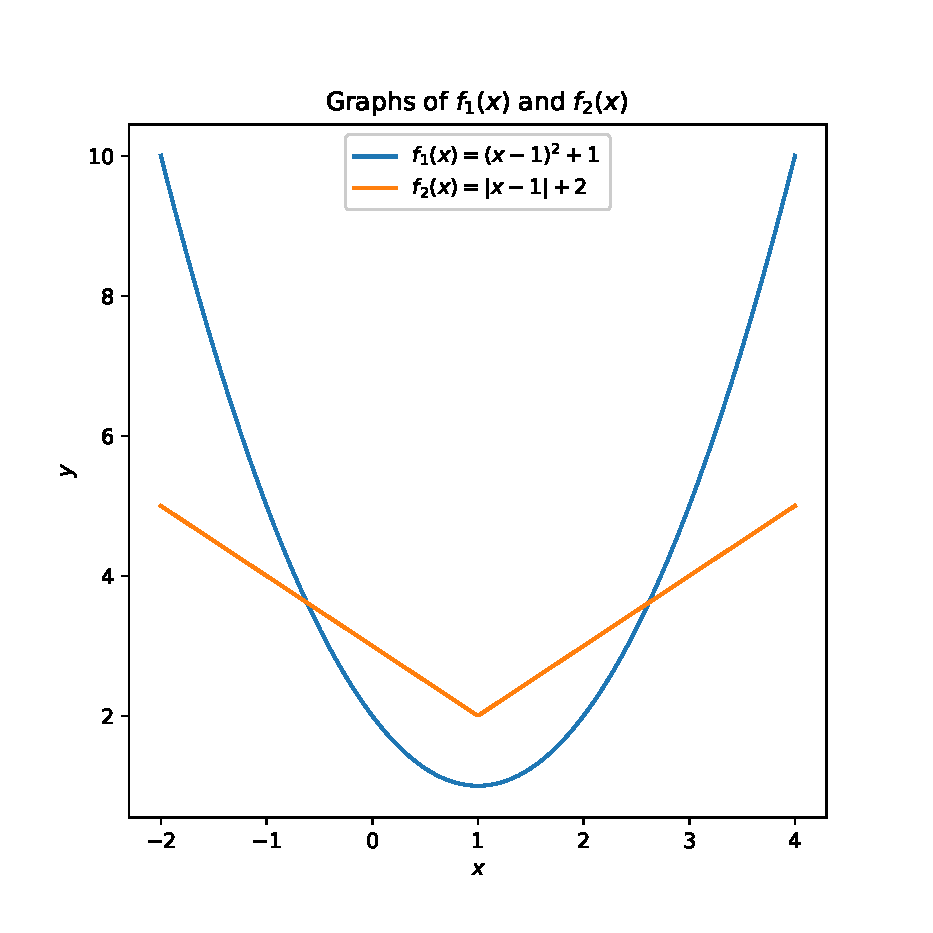
\includegraphics[scale=0.3]{figure1.eps}
		\hspace{1in}
		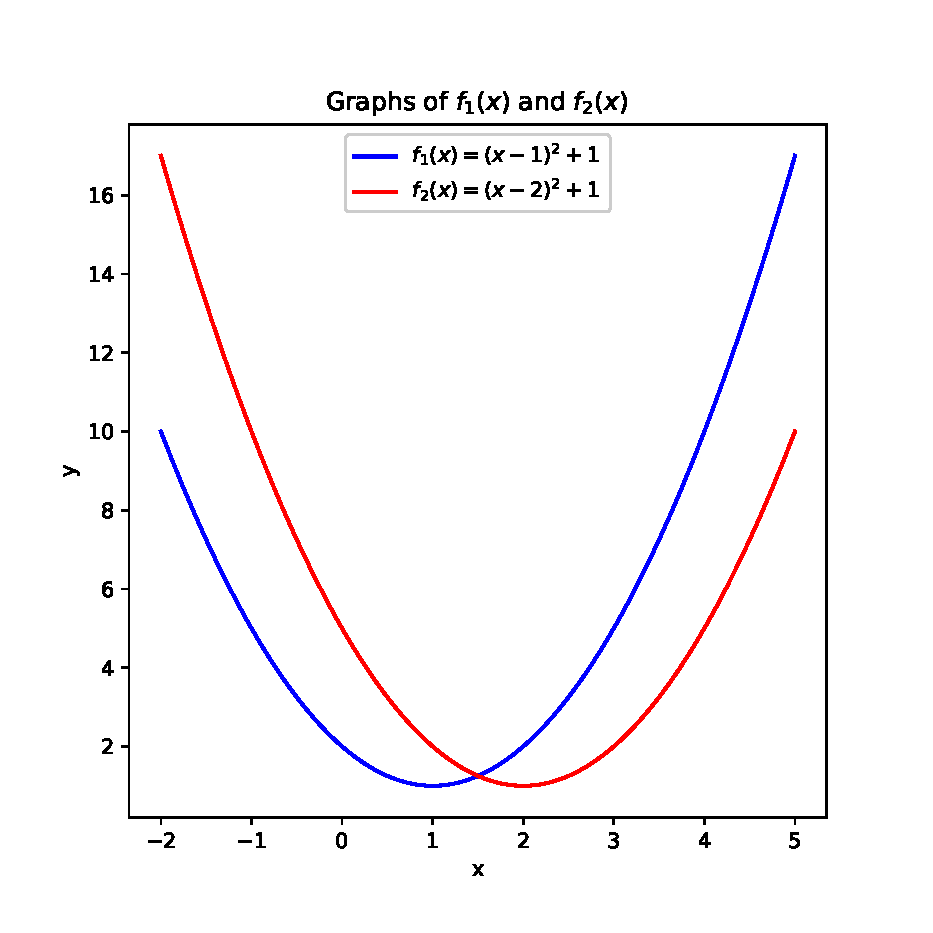
\includegraphics[scale=0.3]{figure2.eps}
	\end{figure}
		
	
	\end{frame}
	\begin{frame}
		\frametitle{权重系数变化法}
	给每一个子目标函数$f_i(x)$赋予权重$w_i$,将$u[\,f \,](x)=\sum_{i=1}^{p}w_i f_i(x)$作为评价函数,将其转化为单目标优化问题.权重系数变化法就是在此基础上对每个个体取不同的权重系数,用通常的遗传算法求解多个Pareto最优解.
		
	
	\end{frame}
	\begin{frame}
		\frametitle{并列选择法}
		\begin{tikzpicture}[node distance=10pt]
  			\node[draw]                      (step 1)  {按子目标均分成子群体};
  			\node[draw, below=of step 1]                        (step 2)  {每个子群体分配一个子目标进行选择运算};
			\node[draw, below=of step 2]                        (step 3)  {挑出适应度高的个体组成新子群};
  			\node[draw,below=of step 3]       (step 4) {合并成完整群体进行交叉,变异运算};
  			\node[draw, below=of step 4]                   (step 5)  {生成下一代};
  		
  
  			\draw[->] (step 1) -- (step 2);
			\draw[->] (step 2) -- (step 3);
			\draw[->] (step 3) -- (step 4);
			\draw[->] (step 4) -- (step 5);
			\draw[->] (step 5.east) .. controls +(right:4cm) and +(right:4cm) .. (step 1.east);
  			
		\end{tikzpicture}
	\begin{block}{}
	容易产生个别子目标函数的极端最优解,找到所有函数的协调最优解比较困难
	\end{block}
	\end{frame}

	\begin{frame}
		\frametitle{排序选择法}
		\begin{tikzpicture}[node distance=10pt]
			\node[draw, rounded corners] (start) {开始};
			\node[draw, below=of start]                      (step 1)  {设置初始序号$r\gets 1$};
			\node[draw, below=of step 1]                        (step 2)  {求出群体中Pareto最优个体,定义序号为$r$};
			\node[draw, below=of step 2]                        (step 3)  {从群体中去掉Pareto最优个体,$r \gets r+1$};
			\node[draw, diamond, aspect=2, below=of step 3]                        (choice)  {是否所有个体都已被处理?};
			\node[draw,rounded corners, below=of choice] (end){结束};
			\draw[->] (start) -- (step 1);
			\draw[->] (step 1) -- (step 2);
			\draw[->] (step 2) -- (step 3);
			\draw[->] (step 3) -- (choice);
			\draw[->] (choice) -- node[right] {是}(end);
			\draw[->] (choice.east) .. controls +(right:1cm) and +(right:1cm) .. node[left] {否}(step 2.east);
		\end{tikzpicture}
		
	
	\end{frame}
	\begin{frame}
		\frametitle{排序选择法}
		\begin{block}{基本思想}
			基于Pareto最优个体排序,依据排列次序进行选择运算,使得排在前面的Pareto最优个体有更多的机会遗传到下一代群体中,经过循环得到Pareto最优解.
		\end{block}
		
	
	\end{frame}
	\begin{frame}
		\frametitle{共享函数法}
		\begin{block}{}
			一般希望解分散在整个Pareto最优集合内,而不是集中在某一部分,因此利用小生境遗传算法,让小生境数较小的个体有更多的机会遗传到下一代群体中.增加了群体的多样性.
		\end{block}
		\begin{definition}[小生境数]
			$m_X=\underset{Y\in P}{\sum} s(d(X,Y))$, $s(d)$为共享函数,关于$d$单调递减.
		\end{definition}
	
		
	
	\end{frame}
	\begin{frame}
		\frametitle{共享函数法}
\begin{algorithm}[H]                           % HERE!!!!!!!!!
\caption{Tournament Sharing Selection}          % give the algorithm a caption
\label{alg1}      % and a label for \ref{} commands later in the document
\begin{algorithmic}[1]  % enter the algorithmic environment
	\STATE 给定$k$
	\STATE 群体中随机选$k$个个体组成集合$C$
	\STATE 群体中随机选$2$个个体组成集合$T$
	\STATE 比较$T$中个体于$C$中个体优越关系
	\IF{$T$中一个个体($X$)比$C$中所有个体优越,另一 个体不比$C$中所有个体优越}
		\STATE $X$遗传到下一代
	\ELSE
		\STATE $T$中小生境数较小的个体遗传到下一代
	\ENDIF
	
\end{algorithmic}
\end{algorithm}
\end{frame}
\begin{frame}
\begin{block}{优点}
	能够得到多种不同的Pareto最优解
\end{block}
\begin{block}{缺点}
	需要进行大量评价和比较运算,搜索效率较低
\end{block}
\end{frame}
\begin{frame}
	\frametitle{混合法}
	\begin{algorithm}[H]                           % HERE!!!!!!!!!
		\caption{Hybrid Selection}          % give the algorithm a caption
		\label{alg2}      % and a label for \ref{} commands later in the document
		\begin{algorithmic}[1]  % enter the algorithmic environment
			\STATE \textbf{并列选择过程}:按子目标个数将群体均分成子群体,并产生下一代子群体
			\STATE \textbf{保留Pareto最优个体过程}:子群体中的Pareto最优个体不进行交叉,变异运算,直接保留到下一代子群体
			\STATE \textbf{共享函数处理过程}:将子群体中非Pareto最优个体组成集合,进行共享函数选择运算,产生下一代子群体
		\end{algorithmic}
	\end{algorithm}
		\begin{block}{主要思想}
			主体使用并列选择法,通过引用保留最佳个体和共享函数的思想弥补并列选择法的不足.
		\end{block}
	

\end{frame}
\begin{frame}
	\frametitle{算例}
	\begin{block}{算例}
		\begin{eqnarray*}
			&\min f_1=x_1^2/4\\
			&\min f_2=x_1(1-x_2)+5\\
			&\textbf{s.t.} \left\{ \begin{array}{c}
				1\le x_1 \le 4\\
				1\le x_2 \le 2	
			\end{array} \right.
		\end{eqnarray*}
	\end{block}
	\begin{block}{}
		变量用8为二进制编码串表示,交叉运算使用单点交叉算子,变异运算使用基本位变异算子.\\
		运行参数为:$ \{ M,T,p_c,p_m \} = \{ 100,100,0.8,0.01 \}$
		
	\end{block}

	

\end{frame}
\begin{frame}
	\frametitle{结果}
\begin{figure}[htbp]
	\centering
	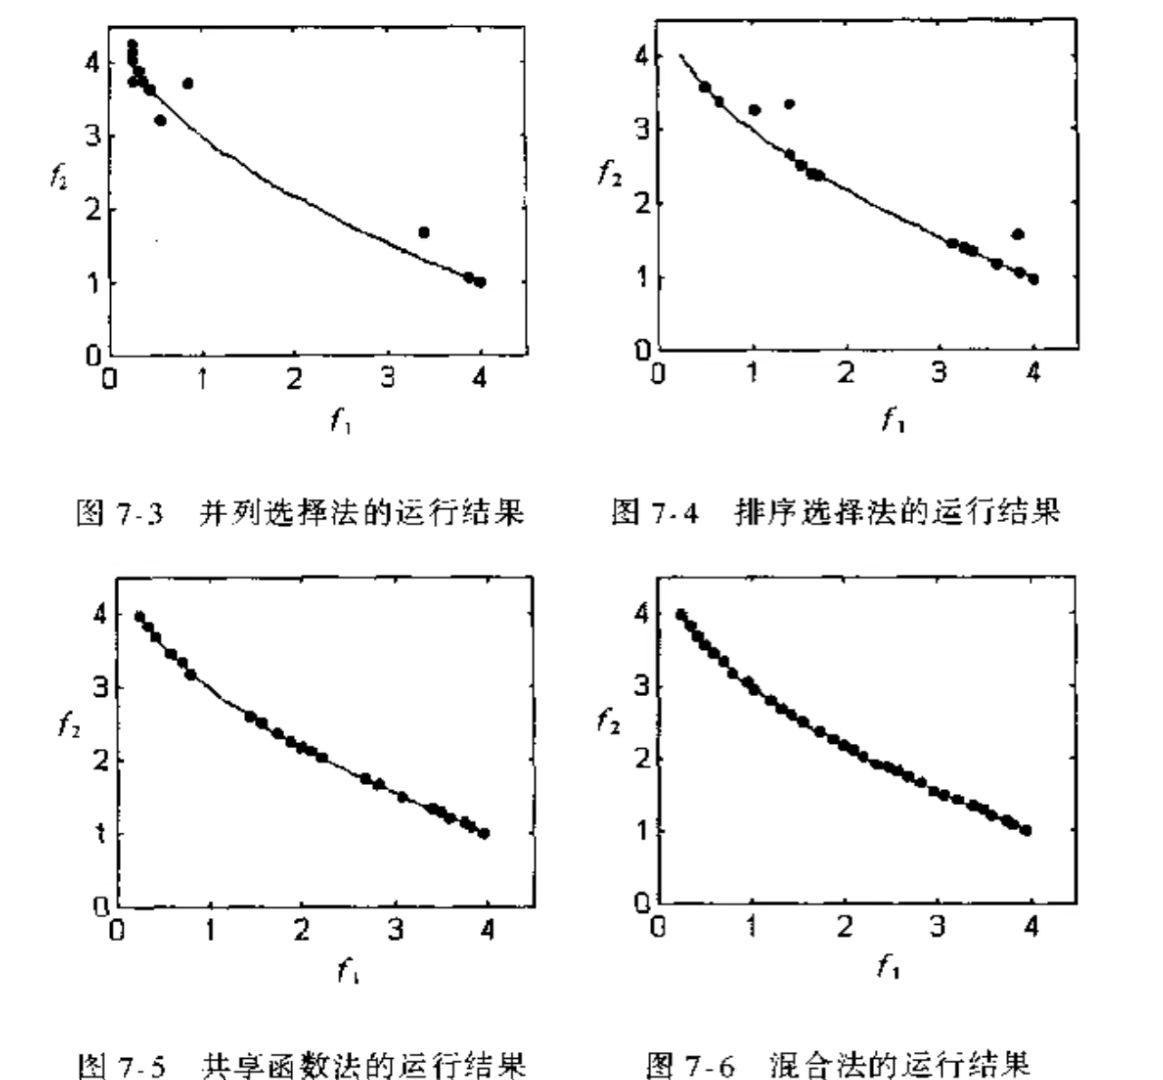
\includegraphics[width=0.6\textwidth]{计算结果.jpg}
\end{figure}
\end{frame}
\begin{frame}
	\frametitle{测试}
	\begin{figure}[ht]
		\centering
		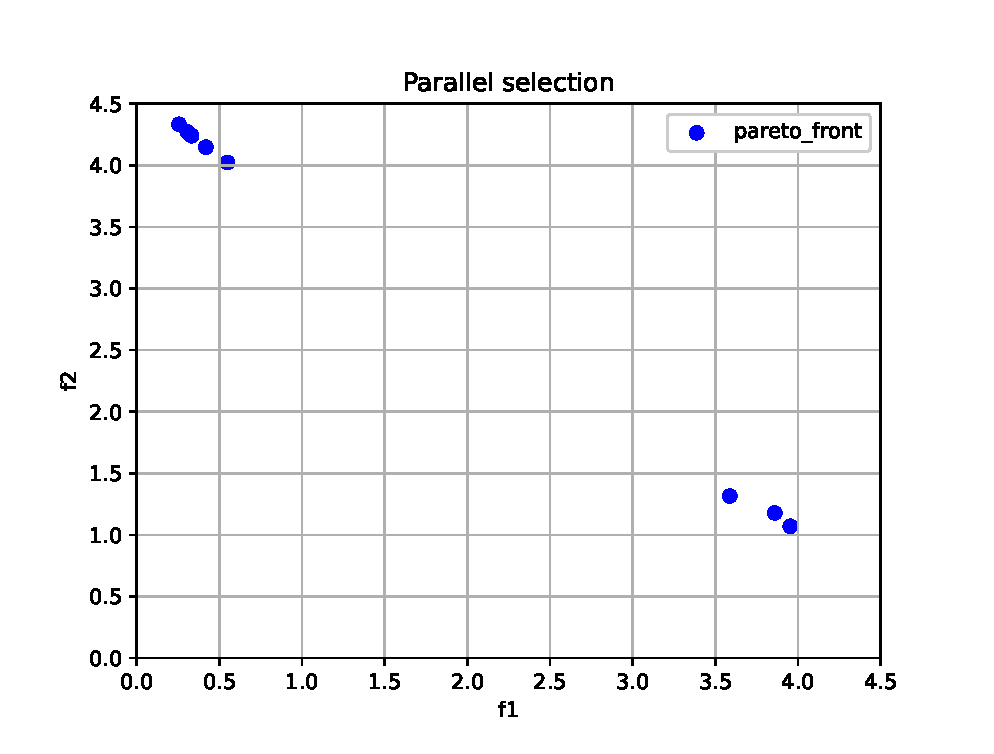
\includegraphics[scale=0.3]{parallel.eps}
		\hspace{1in}
		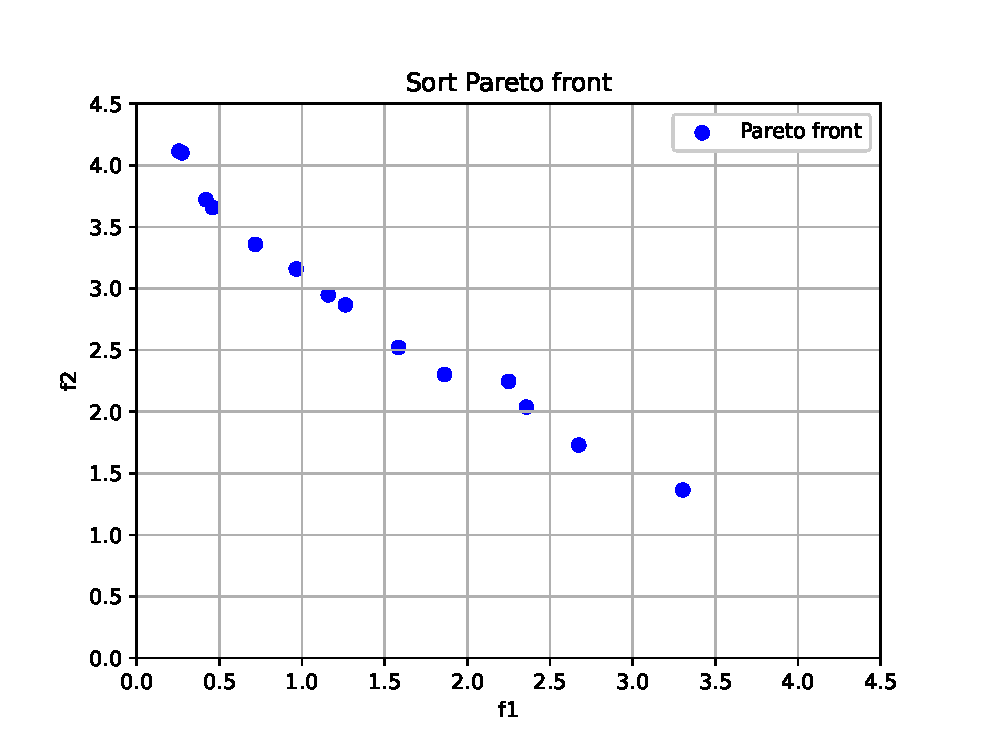
\includegraphics[scale=0.3]{sort.eps}
	\end{figure}
\end{frame}
		
	
	%------------------------------------------------
	

	%------------------------------------------------
	

	
	\begin{frame}
		\Huge{\centerline{Thank you all!}}
	\end{frame}
	
\end{document} 
